\subsection{Dojo Funktion}


\subsection{Dojo Aufbau}
Das Design des Dojos aus Abbildung \ref{fig:DojoBild} wurde für die Batcherorarbeit von Jana Kalbermatten erarbeitet und dient als Vorlage für das Gerät. Der Dojo ist mit $245mm$ ziemlich lang, besitzt jedoch mit einem Aussendurchmesser von nur $19.5mm$ einen kleinen Querschnitt. Dieses Gehäuse setzt eine detailierte Planung der elektronischen Bauteile voraus, sowie ein kompaktes Design der elektronischen Schaltung.


\begin{figure}[h]
	\centering
	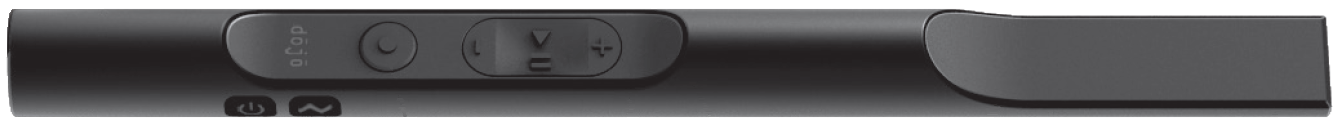
\includegraphics[width=\textwidth]{graphics/DojoBild.png}
	\caption{Aussenansicht des Dojos}
	\label{fig:DojoBild}
\end{figure}

Durch den begrenzten Durchmesser und der begrenzten Schiebeöffnung auf der Rückseite des Dojos kommen keine Akkumulatoren der Normgrösse $A$ sowie $AA$ infrage. Eingebaut wird daher ein Akkumulator der Grösse $AAA$. Um mit den Tastern und dem USB-Port nicht in konflikt zu geraten, wird der Akkumulator in der Mitte des Dojos eingebaut siehe Abbildung \ref{fig:DojoQuerschnitt}. Dies hat ebenfalls den Vorteil, das man einen Print der Länge $120mm$ einbauen kann, der den USB Port, sowie alle Taster beinhaltet.

\begin{figure}[h]
	\centering
	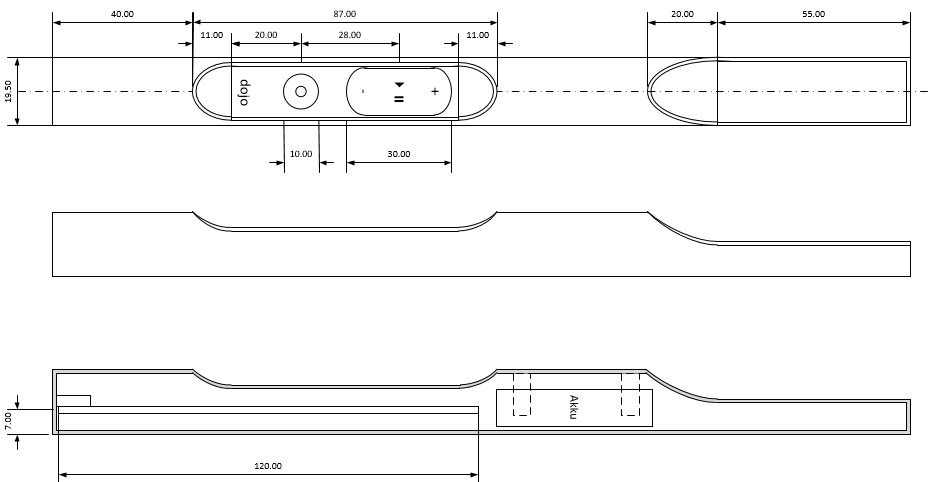
\includegraphics[width=\textwidth]{graphics/DojoQuerschnitt.png}
	\caption{Technische Zeichnung des Dojos}
	\label{fig:DojoQuerschnitt}
\end{figure}